\subsection{Automatic Format Inference}
\label{ssec:format-inference}

When a network problem, compromised machine or malfunctioning application
has been discovered, tracing the problem or attack to
prevent a recurrence is imperative.  This forensic analysis involves
human-guided study of multiple data sources such as log files and
other audit trails.  These data sources are great stores of
information, but they come in many varied and complex forms. They can
contain errors, either unintentional or malicious, and they can be
very, very large.  

To perform forensic analysis, analysts need to quickly understand a
variety of data sources and to ask specific questions about their
contents.  The variety, volume, and complexity of the data mean that
analysts need computational tools to support their analyses and to aid
in information extraction.  However, since every system is different
and the variety of data is so extensive, it is impossible to build
proactively all the specific tools one might need.

In the case of an attack, network forensic analysis should be done in
real-time, perhaps even while an attack is still underway. Not only
does this timeliness increase the chance of discovering the attacker
directly, it also provides the opportunity of identifying and
isolating compromised machines so that the attack cannot spread
further.  Of course, even in the case where an attack or problem is not
deemed urgent, a system adminstrator's time is always valuable --
improvements in administrator efficiency will be translated into 
improvements in their employer's bottom line.

Thus forensic analysts face a twofold problem: (1) they must be able
to ask questions of a wide array of data sources, impossible to
predict in advance, and (2) they must do so highly efficiently.  If
analysts faced only problem (1), they might take their time building
custom tools to query each individual data source from scratch, 
a task that might involve parsing, query support, and visualization 
components.  If analysts faced only problem (2) for a single data source 
known well in advance, they might take the initiative to develop a 
single, standard tool.  Our challenge is to solve both (1) and (2) 
simultaneously: to provide a platform for rapid generation of 
parsing, querying and visualization components for new and evolving
application data sources.

Although PADS descriptions can make managing ad hoc data much easier,
the problem of producing the description in the first place
remains. Writing such descriptions can be tedious and time consuming,
often requiring iteration. First, analysts write a description of as
much of the data as they understand. From this description, they
generate and run analysis tools to find any unknown parts of the
data. They then study those parts and refine the description
accordingly. They repeat this process until all the data either
conforms to the description or constitutes an error in the data rather
than an error in the description.  While the web server log we displayed
earlier may seem easy enough to describe by hand, it is amongst the
simplest examples that we could choose -- application logs may be much
more involved, requiring two-, three- or five-fold more complex descriptions.  
Moreover, the complexity of the situation grows tremendously in a realistic
setting where one must deal with logs of huge size (millions of lines long)
or large archives of logs of many different kinds. 
Having a tool to help produce such descriptions and to generate
data transformation and analysis tools automatically would speed up
forensic analysis and investigation efforts enormously.

\subsubsection*{Format Inference and Tool Generation Architecture}

\begin{figure}
\begin{center}
\centerline{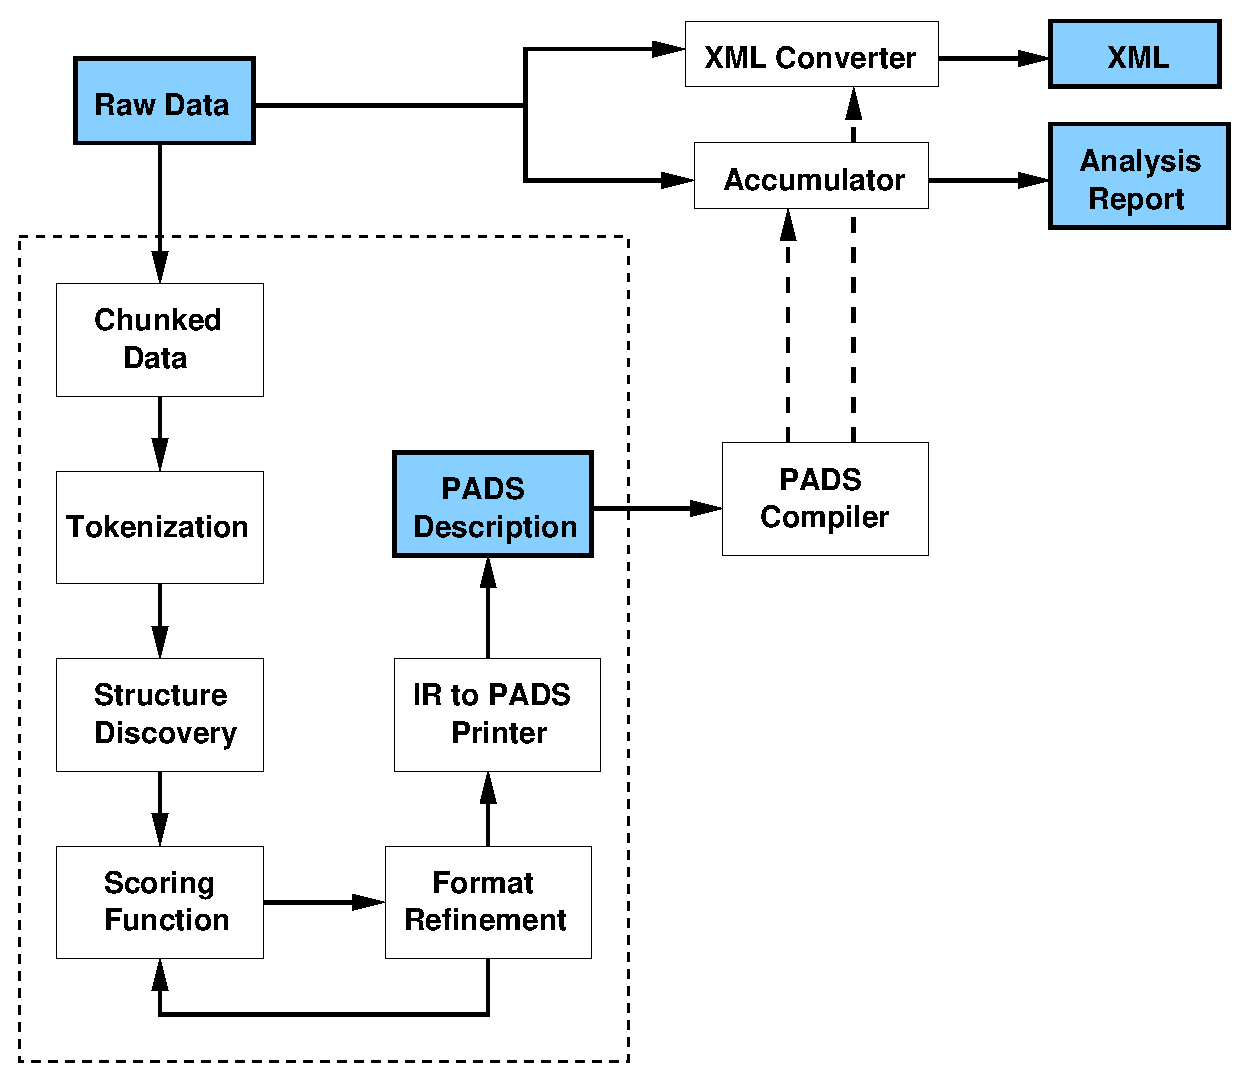
\psfig{file=format-inference-engine.eps,height=2.5in}}
\end{center}
\caption{Modular Architecture of a Format Inference and Tool Generation Engine}
\label{fig:format-inference-engine}
\end{figure}

In preparation for this proposal, we have begun to build a tool for
automatic format inference and data analysis tool generation.  In the
course of building this prototype we have defined a promising, modular
architecture for solving the problem and performed some preliminary
experiments.  Our preliminary experiments have revealed the fact that
our proposal is indeed feasible yet many important challenges must be
overcome to turn our prototype into a robust, precise and viable
system.

The overall architecture we proprose is presented in
Figure~\ref{fig:format-inference-engine}.  As the diagram shows, the
system takes raw data (sets of systems or application logs) as an
input, pushes the raw data through the inference engine and generates
a \pads{} description.  This description is then automatically fed
through the \pads{} compiler to produce several simple
data-processing tools including a tool that will read in the data and
translate it to \xml{} as well as a tool (listed in the diagram
as ``the accumulator'')
that will read in data and output a simple statistical overview,
which includes the distributions of values in each data field and
the number of errors that it finds.

The heart of the proposal is a highly modular, multi-phase inference 
engine.  These phases include:

\begin{itemize}
\item {\bf Chunking:}  The first step in the inference process
is to break data into pieces, with the goal that each piece will have
a similar repetitive structure.  Currently, a user can manually
specify that the data should be chunked line-by-line or file-by-file.
However, we also envision handling several other
chunking strategies including paragraph-by-paragraph chunking or
directory-by-directory chunking of data sets.  Moreover, when the
chunking structure when it is unspecified, we will need to research
heuristics capable of discovering appropriate chunking strategies.

\item {\bf Tokenization:}  
The contents of every chunk of data must be divided up
into {\em tokens} such as numbers, words, punctuation, dates, times, 
ip addresses, phone numbers, etc.  Our current prototype includes built-in
support for a small number of basic tokens.  Our preliminary 
experiments indicate
effective tokenization is an extremely important element of the design, yet
astonishingly hard to achieve due ambiguities that arise in token definitions.
In particular, the {\em local} tokenization techniques we are currently using
seem insufficient for disamiguation in general and we are eager to investigate 
techniques that use more {\em global} information to achieve more precise,
comprehensive and useable tokenization strategies.

\item {\bf Structure Discovery:}
After tokenization, the structure discovery phase produces a
candidate format for the data being analyzed.  This candidate is
produced through a recursive divide-and-conquer algorithm that uses
various heuristics to split the data into subpieces. These
subpieces are analyze and formats for them are generated.
The resulting formats are combined to create an overall description. 
 
Our prototype divide-and-conquer algorithm
works well in some cases but in other cases fails, producing \pads{} 
descriptions that do not parse all of the data in the test set.
The reason for this failure is that not all \pads{} features will 
{\em compose} properly with one another.\footnote{Technically, the
inference algorithm requires
that if $D_1$ and $D_2$ are \pads{} descriptions, then the language of their
concatenation $L(D_1 . D_2)$ must be equivalent to the concatenation
of their languages $L(D_1) . L(D_2)$.  When this property holds our
recursive divide-and-conquer algorithm always succeeds.  We require
similar compositionality properties for union and Kleene star.}  
While such compositionality properties are easy to achieve when dealing with
context-free grammars, \pads{} contains context-free and 
{\em non-context-free} features
such as the ability to read an integer $k$ from a data source
and then parse some element $k$ times (a crucial feature for reading
almost any binary data format).  Such features allow one to
write classic non-context free formats such as $a^k b^k c^k$.
Hence, in order to develop a robust tool generation engine, we must
investigate how to redesign several of the core elements of 
the \pads{} language and implement them efficiently, an important
theoretical and implementation challenge.

\item {\bf Scoring Function and Format Rewriting:}
The format generated by the structure discovery phase is only a 
rough {\em guess}
at the structure of a format.  It is often unnecessarily complicated
in some places and too limited in others.  In order to improve the 
quality of the guess, we {\em score} the format and then search for ways
to optimize it using a collection of format rewriting rules.  The
score is based upon the information-theoretic principles embodied in
the Minimum Description Length Principle (MDL)~\cite{mdl}.  In our
experience to date, this format rewriting is somewhat effective --
it reduces the score of the formats initially produced substantially.
However, to the human eye, much improvement can still be made.  We must
investigate the sources of the problems, develop new rewriting rules
and refine the scoring function, which determines which rules to apply and
when. 
\end{itemize}

In addition to further studying, evaluating, and improving each of the phases
of the inference engine mentioned above, we will engage in two additional
tasks with regards to this element of the grant:

\begin{itemize}
\item {\bf Scaling to large data sets:}  Our initial proof-of-concept was 
designed for small log files on the order of 1000-3000 lines of code.
This proof-of-concept loads all of the data into memory and employs
a variety of relatively expensive algorithms to analyze it during the
structure discovery, scoring and rewriting phases.  New research is
required to scale the system up to handle realistic log files millions
of lines long (or longer).  We believe the key to doing so is to invent
new {\em incremental} versions of our algorithms capable of 
processing large files by iteratively applying more expensive
algorithms on small, manageable chunks.  The research challenges
involved in this endeavor include (1) techniques for summarizing
information discovered in one small chunk and passing it on to the
next, (2) techniques for effectively and
efficiently merging the results of format inference on small chunks
to create an overall description, and (3) analyzing the complexity and
improving the efficiency of existing algorithms.

\item {\bf Holistic repository inference:}  Our initial proof-of-concept
was also designed for determining the structure of a single log file.
However, a single application will often generate multiple different
sorts of logs -- for performance monitoring, for debugging, for 
historical analysis and for exceptional circumstances.  Moreover,
sets of applications will create sets of logs.  All of these logs
will be organized in repositories spanning multiple directories.
Hence, we will also explore new techniques for analyzing the contents
of entire directories and their subdirectories.  Our new techniques
will seek to explain the structure of a repository and present it graphically
to the user for further analysis and mining.

\end{itemize}

\paragraph*{Summary of Format Inference Research:}  
In preparation for this proposal, we have developed a prototype
format inference engine and tool generation system for log files.  
This prototype demonstrates
the viability of our approach.  However, all phases of
our prototype inference engine (chunking, tokenization, structure discovery,
scoring and rewriting) must be further researched and 
improved in order to deliver a reliable and
effective automatic tool generation engine.  Moreover, our preliminary
research has shown that
the basic pads engine does not possess the necessary {\em compositionality
properties} to support our divide-and-conquer inference algorithm in all cases.
Both theoretical and practical research is necessary to design and
implement a new, efficient engine with the appropriate compositionality
properties and the ability to support the required non-context free features.
In addition to these tasks, we must develop
completely new algorithms in order to scale our current system up to 
be able to handle application log files and sets of log files
of realistic size and complexity.
Finally, we must develop new techniques to extend the scope of our engine
so that it can analyze and uncover the structure
of entire repositories full of log files.